\section{Discussion} \label{sec:Discussion}
\subsection{Implications}
\textcolor{red}{Fazit + implications of my results in the bigger picture of research and science}
\\\\\textbf{Cold vs hot streams:}
The assumption that the \ac{DF} of accreted particles is a $\delta$-function in action space requires them to be on the same orbit - an assumption that is not fully \textcolor{red}{reference} but more closely \textcolor{red}{reference} satisfied for cold stellar streams. Already in the introduction we have mentioned, that \ac{DG} mergers usually create hot stellar streams so our particle streams in Auriga are dynamically hot and have a different, more complex \ac{DF}.

\subsection{Comparison to observations\textcolor{red}{better title}}
It is import to compare results from analysis simulations to observations. One test is looking at our Galaxy, where we have 6D phase space information available, e.g. with Gaia \citep{Gaia...mission...2016, GaiaDR2...overview...2018}, and to see how remnants of a \ac{DG} merger are distributed actions space.
\iffalse
\textbf{Excursion: coordinate transformations}
private communication with Wilma Trick
\fi
Recently, \textit{Gaia}-Enceladus \citep{Enceladus....Helmi...2018} \textcolor{red}{also put in references of sausage DG} was discovered in the \textit{Gaia} data. These are remnant stars of a merger approximately \SI{10}{Gyr} ago with a mass ratio of 0.24. In contrary to the Sagittarius \ac{DG} we have precise 6D information from \textit{Gaia} DR2 about Enceladus which we need to calculate the actions. The time of its merger is comparable to prog4.\textcolor{red}{more info on enceladus: what data; selection; coordinate trafo; potential assumption; discovery of enceladus}

\begin{figure}[htbp]
    \centering
    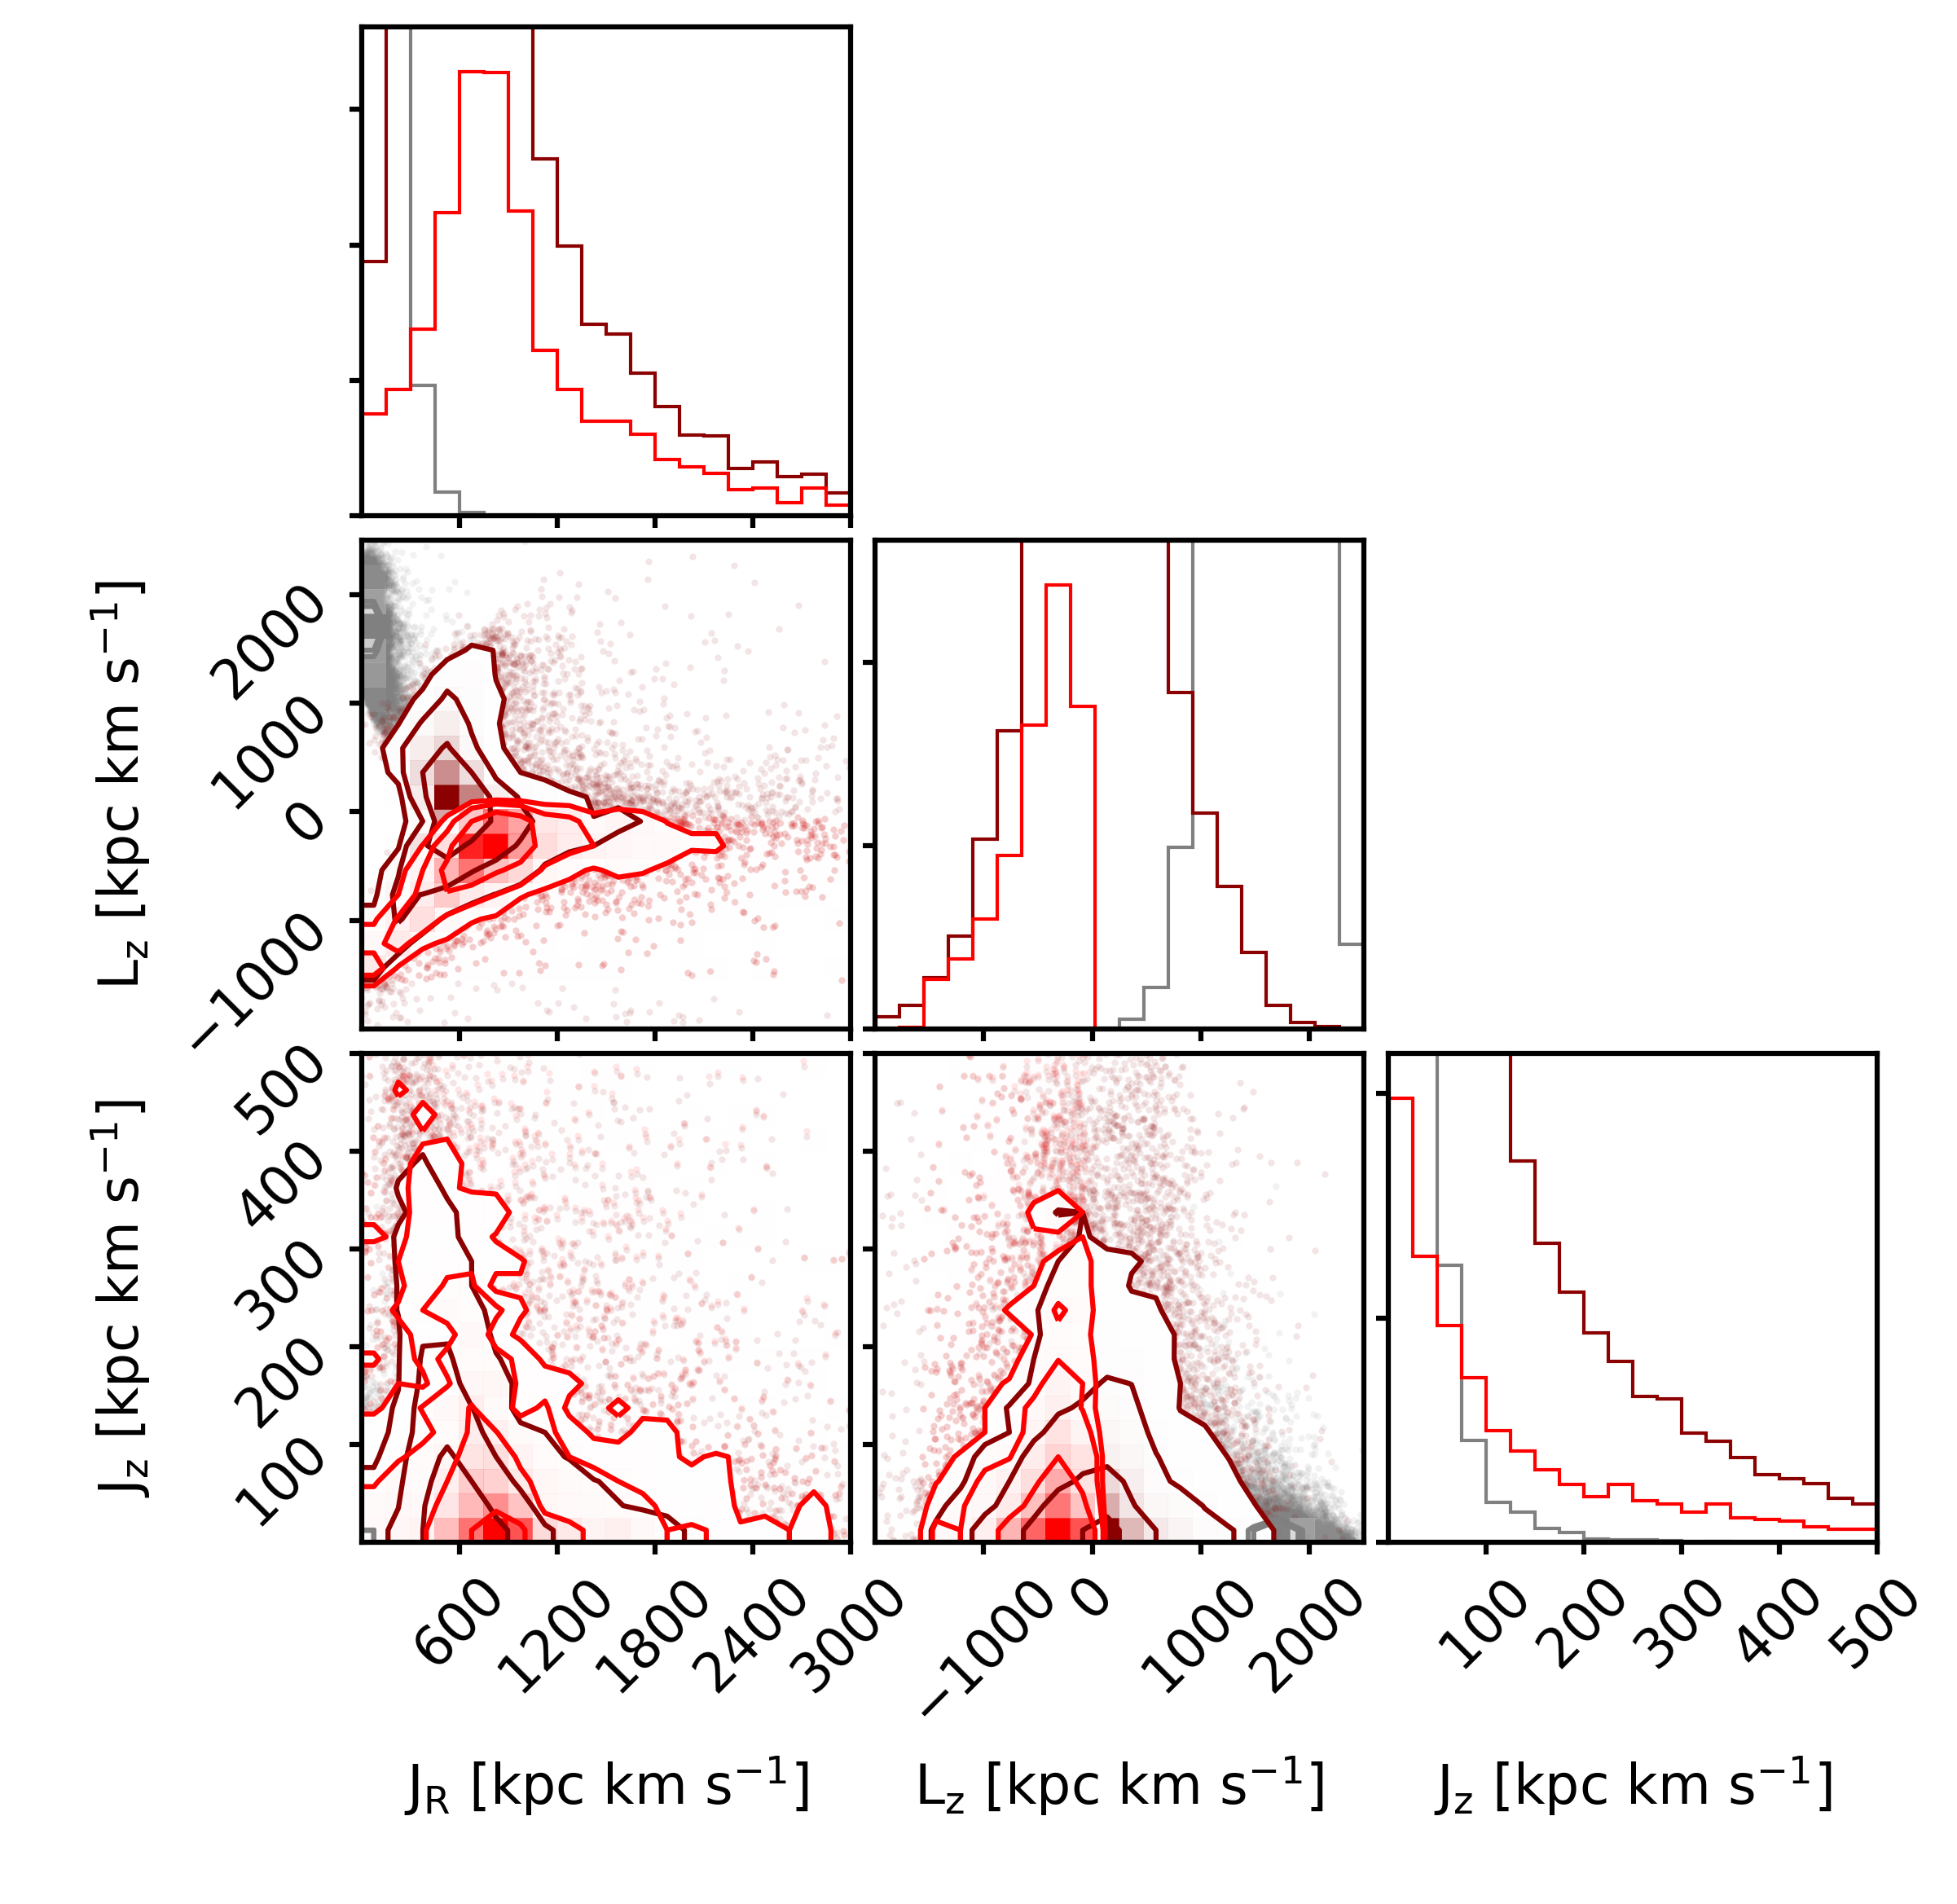
\includegraphics[width=1.0\textwidth]{plots/Discussion/Gaia_all_actions_MW14_talk3.png}
    \caption{\textit{Gaia}-Enceladus stars in action space in the MWPotential2014 \citep{Bovy...galpy...2015}. The data is taken from \textit{Gaia} DR2 \citep{GaiaDR2...overview...2018} in the \ac{MW} within \textcolor{red}{what distance $1/\omega <...kpc$}In grey, actions of disk stars are plotted. Dark red is the halo including some of the thick disk stars. \textit{Gaia}-Enceladus stars are plotted in red. Disk and halo are clearly distinguishable in angular momentum and also in radial action. \textit{Gaia}-Enceladus is not distinguishable from the halo as it makes up a significant part of it. It has a negative $L_z$ therefore it is counterrotating. It is also very spread out in action space so we cannot detect any sharp features.}
    \label{fig:Gaia_Enceladus_actions}
\end{figure}
We show in Figure \ref{fig:Gaia_Enceladus_actions} actions of the disk, halo and \textit{Gaia}-Enceladus. The remnants are neither distinguishable from the halo nor do they make a sharp feature in any of the actions. This tells us that even if there was more dynamical information contained in these stars shortly after the merger, this information vanishes over time. This confirms our findings that actions of objects accreted from a \ac{DG} merger cannot be seen as sharp features after some evolution. 


\subsection{Context in recent research and literature}
\textbf{\acp{GC} formation in cosmological simulations} Timo Halbesma (PhD student at the MPA) is working on extracting \acp{GC} in the Auriga simulations which have proper physical properties and physically motivated formation recipes. Repeating the same analysis in this work with a set of proper \acp{GC} could change our results. One reason could be that if we select properly surviving \acp{GC} they could clump in action space because their orbits might stay constant and therefore they could be used to tune the potential right.\\
The E-MOSAICS simulation suite \citep{Pfeffer...E-MOSAICS...2018, Kruijssen...E-MOSAICS.MW..2018} are zoom-in simulations of the cosmological EAGLE \citep{Schaye...EAGLE...2015} simulations which have implemented models describing the formation, evolution, and disruption of star clusters. In these simulations, Meghan Hughes (PhD student at ESO/LJMU) works on modelling the potential and Sebastian Trujillo-Gomez (Post-doc at ARI) investigates the kinematics of the \acp{GC}. 
\\\\
\textbf{Constraining gravitational potential}
\textcolor{red}{sorry muss hier noch in die literatur schauen}
There are attempts of applying adaptive dynamics or dynamical modelling with \acp{GC} to the \ac{MW}.
\begin{itemize}
    \item \textbf{\acp{DF} of \acp{GC}} \citep{Posti...MWmassGCs...2018}
    looked at all GCs and did not differentiate bw in-situ/ex-situ and coming from differetn \acp{DG}
    \item \textbf{Sharpen stellar streams in sims to find true potential} \citep{Sanderson...streams..adaptivedyn...2015, Sanderson...gravpotstreams...2017}
\end{itemize}
\citet{Jean-Baptiste...accactionspace...2017}

\subsection{Caveats}
\textcolor{red}{too harsh}This work and its results cannot be blindly trusted. There are a few assumptions and problems in the course of the investigations which might have influenced the results.
\\\\\textbf{GC selection:}
One of the main problems in the analysis is the \acp{GC} selection. Auriga does not resolve \acp{GC} and therefore we need to make assumptions and select \ac{GC} candidates. We applied a very simple recipe which only excluded simulated particles as \ac{GC} candidates which were in a snapshot in a regime where the stellar disk was very dense \textcolor{red}{Wilma has an idea how to show strong disk forces; if time ask her} and could have destroyed the \ac{GC} \textcolor{red}{reference for GC destroyed in disk}. \textcolor{red}{check the next sentence; try to better describe the specific not random selection} When selecting only a subset of the \acp{GC}, we have very different statistics of each progenitor group, e.g. the means shift significantly. A proper, physical selection would make these results more reliable. \textcolor{red}{what could be considered in the physical selection of GCs and why is this not in Auriga}
\\\\\textbf{Potential fit:}
As we have discussed in Section \ref{subsec:wrong_pot_fit}, there are a few problems with the potential fit. The bulge-disk decomposition probably underestimates the disk and creates a flaring spatial selection effect. For each component, the model differs from the data especially in the center. This is due to the choice of binning the data, fitting routines, the assumption of spherical or axisymmetry, the simplified potential model consisting of only three analytic building blocks etc. In total, the potential is good enough for the course of our investigations but, as one of the next steps, should be improved.

\subsection{Future Work}
There are a lot of things which we could not investigate or we had to make compromises on due to the time limitations of this thesis. Big issues which we already discussed are with the potential model and with the \ac{GC} selection. Improving these recipes would make our analysis more robust. \textcolor{red}{ideas on improvement; check if/what i have mentioned in sec 2.3 and repeat it quickly}
\\\\
galpy and AGAMA \citep{Vasiliev...AGAMA...2019} can in principle calculate actions for \textit{N}-body simulations directly without the need of an analytic gravitational potential. We should compare if the action distribution and evolution behaves as we measured because of their nature and their physical evolution in the simulation (so direct calculation of actions and calculating them in the potential model would give similar results) or because a analytic axisymmetric potential (in general or only our fit) cannot well describe the real potential and messes these things up. Up to now, it was not possible to do this step because of technical issues. 

\\\\The final goal would be to find the right \ac{DF} of accreted particles which is not yet possible due to numerical (and observational) limitations. If we had that, adaptive dynamics in external galaxies should be a useful method to constrain their gravitational potential. With this true \ac{DF} and the right gravitational potential, we would know everything about the dynamics of the galaxy.

